\paragraph{}
Le besoin est né du constat de la lourdeur de processus existants.
Une solution existe mais ne satisfait pas.

D'une part, les personnes à la base des besoins métiers souffrent de résultats mitigés et longs à attendre.
D'autre part, les développeurs doivent exécuter des demandes dont les exécutions sont manuelles et répétitives.

\paragraph{}
La ligne directrice sera donc d'automatiser de manière complète des processus existants et de faire en sorte qu'ils
puissent être menés à bien par la seule personne ayant besoin du résultat de ces processus.

\section{Élaboration}
\label{sec:elaboration}

    \section{Élaboration}
\label{sec:elaboration}

L'élaboration de ce cahier des charges s'est faite en deux phases. 
Dans un premier temps, j'ai participé à des réunions avec Grégory, Renaud et Sophie afin de démarrer le projet. 
Et dans un second temps, nous avons ajouté et adapté des fonctionnalités au fur et à mesure que le projet a avancé.

\paragraph{}
Altissia travaille selon les principes agiles\fnmark et plus précisément la méthodologie SCRUM\fnmark.
Ces principes sont nés d'un constat sur les projets informatiques, pour la majorité échoue\cite{standish_standish_nodate} et la plupart du temps c'est parce que les besoins sont mal définis ou parce que la communication entre les parties prenantes est mauvaise (voir figure \ref{fig:why-projects-fails}).

\begin{figure}[ht]
    \centering
    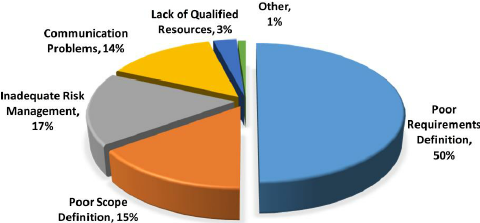
\includegraphics[scale=.8]{images/why-projects-fail.png}
    \caption{Role of Requirements in Software Project Failures. Source: ESI International Survey of 2000 Business Professionals, 2005.}
    \label{fig:why-projects-fails}
\end{figure}

\fntext{Dans le contexte du développement logiciel, l'agilité définit un cadre de travail\cite{noauthor_methode_2018}.
Un point central est le développement par itération dont chacune produit un résultat critiquable par le client.
Ceci a pour but de limiter les efforts potentiellement perdus si le résultat ne correspond pas aux attentes.}
\fntext{Une méthode Agile spécifique qui a la particularité d'organiser le travail sous forme d'échéances à court termes et répétées que l'on appelle les sprints\cite{noauthor_guide_2013}.}

\paragraph{}
Pour répondre à ces enjeux, le service informatique d'Altissia a adopté la méthode SCRUM.
Cela consiste à travailler de manière itérative, de produire des résultats intermédiaires utilisables fréquents, d'impliquer les différents acteurs, d'obtenir leurs commentaires et d'adapter la direction du projet selon ceux-ci.

\paragraph{}
C'est donc pour cela que le cahier des charges n'est pas complet et définitif au début du projet mais qu'il s'étoffe au fur et à mesure.

\subsection{Les interviews}
\label{subsec:interviews}

    En un premier temps, j'ai eu une interview avec Grégory pour définir le besoin général et le contexte qui l'entoure. 
    
    Ensuite, j'ai eu une réunion avec Renaud et Sophie.
    A deux, ils ont défini précisément la problématique des outils existants.
    Renaud connaît très bien l'outil que l'on veut remplacer, Altissia launcher, il m'a expliqué les difficultés rencontrées pendant son développement et comment il a terminé dans son état actuel.
    
    % Elaborer sur les manquements d'Altissia launcher ? On en parle un peu dans l'intro donc pas sur que ça soit nécessaire.
    Sophie a établi quelles sont les manquements du logiciel actuel qu'il faudrait palier et quelles nouvelles fonctionnalités elle voudrait ajouter.

    \paragraph{}
    Une interview avec le directeur technique m'a permis d'établir comment la nouvelle application intéragira avec les applications existantes.

    L'application sera hébergée sur le réseau de travail de l'entreprise.
    Elle doit supporter certaines fonctionalités mais pas l'authentification utilisée par nos microservices en tant que telle.
    Afin de donner accès aux ressources protégées, Altissia créera une version personnalisée\footnotemark de l'application.
    \footnotetext{La personnalisation signifie la reprise du code source afin d'y ajouter les fonctionalités désirées.}

    Ainsi, l'application sera constitué de quatres sortes de composants:
    \begin{itemize}
        \item Une application web cliente Angular qui lui permet d'intéragir avec les utilisateurs.
        \item Une application web server qui permet de communiquer avec les ressources réseaux.
        Celle-ci sera personnalisée afin d'implémenter l'authentification d'Altissia.
        \item Une librairie d'automatisation qui gère l'exécution des tâches et leur journalisation.
        \item Des multiples modules qui chacun permettent de définir une ou plusieurs tâches.
    \end{itemize}

    \paragraph{}
    Renaud, un développeur backend expérimenté, m'a expliqué le défi que sera la libraire d'automatisation de tâches.
    Il faut supporter la définition d'une tâche, l'asynchronicité de son exécution, la possibilité d'exécutions répétées,
    l'utilisation de ressources partagées et la réutilisabilité des tâches.

    Je dois lui proposer une architecture qui permet de relever tous ces défis.

    \paragraph{}
    Sophie, une cheffe de projet qui s'occupe notamment de la publication du contenu des cours et tests de niveaux,
    a défini quel serait le périmètre de l'application.
    Le but est de ne pas implémenter des fonctionalités qui font déjà l'objet de développements prévus ou en cours.

    La fonctionalité qui obtient la priorité pour le moment est la validation du contenu des fichiers Excel des questions du test de niveau.
    Celle-ci est fort demandée et sa complexité est moyenne.
    Elle permettrait de se faire une idée plus précise de ce que l'application pourrait apporter.

    \paragraph{}
    Le directeur technique et moi-même sommes mis d'accord pour une réunion bi-hebdomadaire.
    Je dois organisé une nouvelle réunion avec Renaud pour lui présenter mon plan d'architecture.
    Je verra Sophie dans un moi ou deux pour passer en revue le premier délivrable et discuter des prochains délivrables.

\subsection{Les demandes clients}
\label{subsec:customer-requests}

    La première fonctionalité sera la validation des fichiers Excel des questions de test de niveaux.
    Cette validation comprends les points suivants:
    \begin{enumerate}
        \item La correspondance à une expression régulière.
        \item L'unicité des valeurs au sein d'une colonne.
        \item La cohérence entre deux colonnes (Si la colonne type a la valeur audio, alors la colonne son doit avoir une valeur).
        \item La présence d'une colonne.
        \item L'absence d'impact de colonnes superflues.
        \item L'appartenance à un ensemble de comparaison.
    \end{enumerate}

\subsection{Les propositions au client}
\label{subsec:proposals-to-customer}

    J'ai proposé de n'implémenter que la présence d'une colonne pour la première itération.
    C'est évidemment trop peu pour réaliser un scénario complet mais l'objectif est la mise en place des différents composants logiciels.
    Ainsi, une fois cette première itération accomplie, on pourra juger de la pertinence de la solution choisie.


\section{Lots d'informations identifiés}
\label{sec:identified-information-packages}

    TODO

\section{Les acteurs de l'environnement d'exploitation de l'application}
\label{sec:application-operation-actors}

    TODO

\section{Définition de la première version de l'application}
\label{sec:first-version-definition}

    TODO

\section{Perspectives d'évolution pour une version ultérieure}
\label{sec:future-release-outlook}

    TODO
